\documentclass[a4paper, 12pt, slovene]{article}
\usepackage[slovene]{babel}
\usepackage[utf8]{inputenc}
\usepackage{lmodern}
\usepackage[T1]{fontenc}
\usepackage{graphicx}
\usepackage{caption}
\captionsetup{font=footnotesize}
\usepackage{fullpage}
\usepackage{enumitem}
\usepackage{array}
\usepackage{wrapfig}
\usepackage{multirow}
\usepackage{tabularx}
\usepackage{amsmath}
\usepackage{subcaption}
\newcommand*\diff{\mathop{}\!\mathrm{d}}
\newcommand*\Diff[1]{\mathop{}\!\mathrm{d^#1}}
\newcommand*\difft{\mathop{}\!\ddot{ }}
\usepackage{float}
\usepackage{mathrsfs}

\newcommand{\Ai}{\mathrm{Ai}}
\newcommand{\Bi}{\mathrm{Bi}}

\renewcommand{\Re}{\mathop{\rm Re}\nolimits}
\renewcommand{\Im}{\mathop{\rm Im}\nolimits}
\newcommand{\Tr}{\mathop{\rm Tr}\nolimits}
\newcommand{\diag}{\mathop{\rm diag}\nolimits}
\newcommand{\dd}{\,\mathrm{d}}
\newcommand{\ddd}{\mathrm{d}}
\newcommand{\ii}{\mathrm{i}}
\newcommand{\lag}{\mathcal{L}\!}
\newcommand{\ham}{\mathcal{H}\!}
\newcommand{\four}[1]{\mathcal{F}\!\left(#1\right)}
\newcommand{\bigO}[1]{\mathcal{O}\!\left(#1\right)}
\newcommand{\sh}{\mathop{\rm sinh}\nolimits}
\newcommand{\ch}{\mathop{\rm cosh}\nolimits}
\renewcommand{\th}{\mathop{\rm tanh}\nolimits}
\newcommand{\erf}{\mathop{\rm erf}\nolimits}
\newcommand{\erfc}{\mathop{\rm erfc}\nolimits}
\newcommand{\sinc}{\mathop{\rm sinc}\nolimits}
\newcommand{\rect}{\mathop{\rm rect}\nolimits}
\newcommand{\ee}[1]{\cdot 10^{#1}}
\newcommand{\inv}[1]{\left(#1\right)^{-1}}
\newcommand{\invf}[1]{\frac{1}{#1}}
\newcommand{\sqr}[1]{\left(#1\right)^2}
\newcommand{\half}{\frac{1}{2}}
\newcommand{\thalf}{\tfrac{1}{2}}
\newcommand{\pd}{\partial}
\newcommand{\Dd}[3][{}]{\frac{\ddd^{#1} #2}{\ddd #3^{#1}}}
\newcommand{\Pd}[3][{}]{\frac{\pd^{#1} #2}{\pd #3^{#1}}}
\newcommand{\avg}[1]{\left\langle#1\right\rangle}
\newcommand{\norm}[1]{\left\Vert #1 \right\Vert}
\newcommand{\braket}[2]{\left\langle #1 \vert#2 \right\rangle}
\newcommand{\obraket}[3]{\left\langle #1 \vert #2 \vert #3 \right \rangle}
\newcommand{\hex}[1]{\texttt{0x#1}}

\renewcommand{\iint}{\mathop{\int\mkern-13mu\int}}
\renewcommand{\iiint}{\mathop{\int\mkern-13mu\int\mkern-13mu\int}}
\newcommand{\oiint}{\mathop{{\int\mkern-15mu\int}\mkern-21mu\raisebox{0.3ex}{$\bigcirc$}}}

\newcommand{\wunderbrace}[2]{\vphantom{#1}\smash{\underbrace{#1}_{#2}}}

\renewcommand{\vec}[1]{\overset{\smash{\hbox{\raise -0.42ex\hbox{$\scriptscriptstyle\rightharpoonup$}}}}{#1}}
\newcommand{\bec}[1]{\mathbf{#1}}




\begin{document}

\begin{titlepage}
\title{\textsc{naključni sprehodi} \\[1ex] \large Druga naloga pri predmetu Matematično-fizikalni praktikum}
\author{Gašper Lotrič, 28191019}
\date{23. oktober 2021}

\maketitle
\end{titlepage}

\tableofcontents
\pagebreak


\section{Uvod}
Naključni sprehodi so vrsta gibanja, pri katerem v velikem številu korakov napredujemo iz izhodišča v neko končno lego, tako da se parametri vsakega naslednjega koraka sproti naključno določajo.  Običajni zgled je Brownovo gibanje (difuzija) drobnih delcev barvila po mirujoči homogeni tekočini, kjer je spočetka barvilo zbrano v izhodišču.  ``Težišče'' barvila $\langle x(t)\rangle$ v povprečju ostane v izhodišču, razen če v tekočini vzpostavimo kako anizotropijo (na primer v dveh razsežnostih z vsiljeno rotacijo).  ``Razmazanost'' po dolgem času je sorazmerna s časom,
\begin{equation*}
  \sigma^2(t) \equiv \langle x^2(t)\rangle - \langle x(t)\rangle^2 = 2 D t \>.
\end{equation*}
Sorazmernostni koeficient je običajna difuzijska konstanta, priča smo normalni difuziji.  Ta rezultat izhaja iz
centralnega limitnega teorema (CLT), ki izraža, da je rezultantna porazdelitev končnih leg pri difuziji porazdeljena normalno (Gauss), če so le povprečni časi med koraki in povprečni kvadrati dolžin korakov končni.

Zanimiveje je opazovati naključne sprehode, pri katerih dovolimo nadpovprečno dolge korake.  Verjetnostno gostoto porazdelitve po dolžinah posameznih korakov parametrizirajmo v potenčni obliki
\begin{equation}
p(l) \propto l^{-\mu} \>,
\label{lpow}
\end{equation}
kjer naj bo $1 < \mu < 3$.  Tedaj postane drugi moment porazdelitve
\begin{equation*}
  \langle l^2\rangle = \int l^2 p(l) \dd l
\end{equation*}
neskončen.  Govorimo o anomalni difuziji, prisotni pri celi dru\v zini kinematičnih distribucij dolžin poti z "debelimi repi".

Ustrezno sliko naključnega gibanja, povezanega s temi dolgimi koraki, lahko interpretiramo na dva načina:
\begin{itemize}
  \item L\'evyjev pobeg oz. polet ({\sl flight\/}), implicira, da vsak korak iz porazdelitve~(\ref{lpow}) traja enako dolgo, medtem ko se hitrost gibanja med koraki (divje) spreminja.
  \item L\'evyjev sprehod ({\sl walk\/}), ki interpretira korak iz porazdelitve~(\ref{lpow}) kot  gibanje s konstantno hitrostjo in tako koraki trajajo različno dolgo časa (dolžina koraka je sorazmerna s časom).
\end{itemize}

Slednja intepretacija bolj ustreza fizikalni sliki naključnega gibanja delca skozi snov, medtem ko se prva interpretacija uporablja v druga\v cnih aplikacijah.

Vse naloge lahko obravnavaš za obe interpretaciji, pobegov in sprehodov. V prvem primeru (pobeg, flight) je prete\v ceni \v cas direktno sorazmeren s \v stevilom korakov, v drugem primeru (sprehod, walk) pa je prete\v ceni \v cas  sorazmeren z vsoto dol\v zine korakov.


Pri anomalni difuziji razmazanost (varianca) velike množice končnih leg naključnih L\'evyjevih \textbf{sprehodov (walks)} narašča z drugačno potenco časa.
Velja $\sigma^2(t) \sim t^\gamma$, kjer je
\begin{align*}
1 < \mu < 2 \>, &\qquad \gamma = 2 \> &\qquad&  \text{(balistični režim)}\>, \\
2 < \mu < 3 \>, &\qquad \gamma = 4 - \mu &\qquad&  \text{(super-difuzivni režim)}\>, \\
    \mu > 3 \>, &\qquad \gamma = 1 &\qquad&  \text{(normalna difuzija)} \>.
\end{align*}
Za $\mu=2$ pričakujemo $\sigma^2(t) \sim t^2 / \ln t$,
za $\mu=3$ pa $\sigma^2(t) \sim t \ln t$ (glej na primer \cite{weeks}
in druge reference prav tam).

Slika je nekoliko drugačna pri opazovanju naključnih L\'evyjevih \textbf{poletov (flights)}.
Spet vzamemo zvezo $\sigma^2(t) \sim t^\gamma$ in dobimo odvisnosti
\begin{align*}
1 < \mu < 3 \>, &\qquad \gamma = \frac{2}{\mu-1} \> &\qquad&  \text{(super-difuzivni režim)}\>, \\
    \mu > 3 \>, &\qquad \gamma = 1 &\qquad&  \text{(normalna difuzija)} \>.
\end{align*}
Pri $\mu=2$ očitno pričakujemo $\sigma^2(t) \sim t^2 $, torej balistični režim.
\newline


{\sl Statistični komentar:} v primerih, ko je drugi moment porazdelitve neskončen, bo tudi račun razmazanosti
končnih leg $x_n$ v obliki
\begin{equation}
\sigma^2 = \frac{1}{N-1} \sum_{n=1}^N \left( x_n - \langle x \rangle \right)^2
\label{sig2}
\end{equation}
divergiral oziroma bo imel ob ponovnih zagonih naključnega sprehoda močno raztresene vrednosti.  Pomagaš si lahko na več načinov. širino porazdelitve končnih leg lahko oceniš tako, da prilagajaš Gaussovo krivuljo zgolj centralnega dela porazdelitve, tako da s prilagajanjem ne zajameš štrlečih (ne-Gaussovskih) repov. Lahko tudi neposredno računaš vsoto~(\ref{sig2}), a vanjo vključiš samo ``razumne'' člene (izpusti na primer nekaj odstotkov najmanjših in nekaj odstotkov največjih). Tretja možnost je, da definiramo novo vrsto variance
\begin{equation*}
  \sigma / N^p
\end{equation*}
in poiščemo tako potenco $p$, da ta spremenljivka konvergira za velike $N$ (oz. velike $t$).  še ena možnost je, da vzameš kako robustno mero za množico vrednosti $X_i$, na primer MAD, ``median absolute deviation''
\begin{equation*}
  \mathrm{MAD} \equiv \mathrm{median}_i\left( | X_i - \mathrm{median}_j X_j | \right) \>.
\end{equation*}
Z njo merimo povprečje absolutne vrednosti deviacije na način, ki je zelo malo občutljiv na oddaljene vrednosti v repih porazdelitve, saj te vrednosti na račun mediane bistveno manj vplivajo kot na račun običajne povprečne vrednosti.



\section{Naloga}
Napravi računalniško simulacijo dvorazsežne naključne hoje za \textbf{polete in sprehode}.  Začni vedno v izhodišču ($x=y=0$), nato pa določi naslednjo lego tako, da naključno izbereš smer koraka in statistično neodvisno od te izbire še njegovo dolžino, torej
\begin{eqnarray*}
x &\leftarrow& x + l \cos\phi \>, \\
y &\leftarrow& y + l \sin\phi \>,
\end{eqnarray*}
kjer je $\phi$ enakomerno naključno porazdeljen po intervalu $[0,2\pi]$, dolžina koraka $l$ pa naj bo porazdeljena
v skladu s potenčno obliko (Enačba \eqref{lpow}). Dolžine $l_i$ je v tem primeru potrebno generirati po verjetnostni
porazdelitvi $w(l)\sim p(l)$ (Enačba \eqref{lpow}). Za izra\v cun algoritma je osnova naslednja formula:
\begin{equation}
\int\limits_{a}^{l} w(t)\,  dt = \rho \cdot \int\limits_{a}^{b}  w(t)\, dt,
\label{eq-osnova}
\end{equation}
ki jo je potrebno re\v siti in iz nje izraziti spremenljivko $l$. Tu je $\rho$ (psevdo-)naključno število na intervalu $[0,1]$ ter je $[a,b]$ relevantni interval vzorčenja. Za nekatere porazdelitve je izra\v cun preprost, npr $w(t)=\frac{1}{\tau} e^{-\frac{t}{\tau}}$ nam da kar:
\begin{equation}
l=-\tau \ln(1-\rho).
\end{equation}

V vsakem primeru nariši nekaj značilnih slik sprehodov za $10$, $100$, $1000$ in $10000$ korakov. Iz velikega števila sprehodov z velikim številom korakov nato poskusi določiti eksponent $\gamma$ za nekaj izbranih parametrov $\mu$ oziroma funkcij $f(x)$ v posameznih primerih ter presodi, za kakšno vrsto difuzije gre.



\section{Poleti in sprehodi}
Levyev polet in Levyev sprehod se v 2D trajektoriji ne razlikujeta. Razlike se bodo pojavile šele v naslednjih poglavjih, kjer bo do izraza prišel čas sprehoda. \par\vspace{5mm}

Polete in sprehode sem implementiral v polarnih koordinatah. Dolžine korakov sem generiral skladno z enačbo \eqref{eq-osnova}. Funkcija $w(t)$ mora biti taka, da velja $\lim\limits_{t\rightarrow \infty} w(t) = 0$. Integralsko  mejo $b$ sem poslal v neskončnost, saj je tam $W(t=\infty) = 0$, spodnja meja obeh integralov $a$, pa služi le kot skala problema in sem si zanjo izbral kar $a = 1$. Tako sem dobil porazdelitev za $l_i = W^{-1}(W(a)(1-\rho))$, kjer je $W(t)$ nedoločeni integral $w(t)$. V tej nalogi bom uporabil Pareto porazdelitev $w(l) \propto l^{-\mu}$. \par\vspace{5mm}

V tem delu naloge bom opazoval le izgled 2D trajektorij, zato bom zaenkrat obravnaval le polete. Narisal sem nekaj grafov različno dolgih naključnih poletov pri različnih vrednostih $\mu$.

\begin{figure}[H]
\centering
\begin{subfigure}{0.49\textwidth}
	\centering
	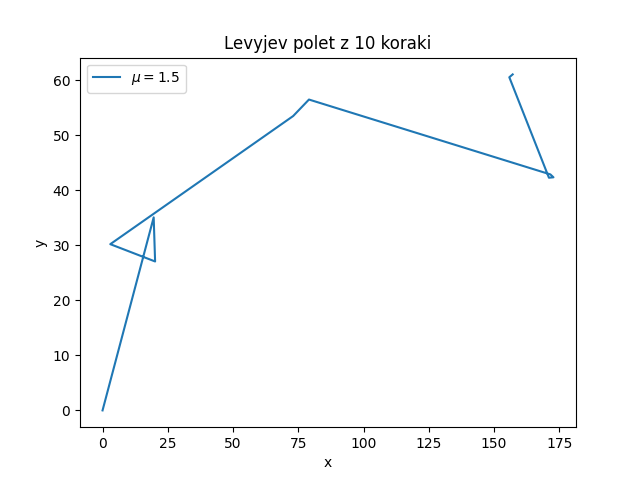
\includegraphics[width=0.95\textwidth]{sprehodi/let-10-1.5.png}
	\caption{2D polet z 10 koraki pri $\mu = 1.5$.}
	\label{fig-let-10-1.5}
\end{subfigure}
\begin{subfigure}{0.49\textwidth}
	\centering
	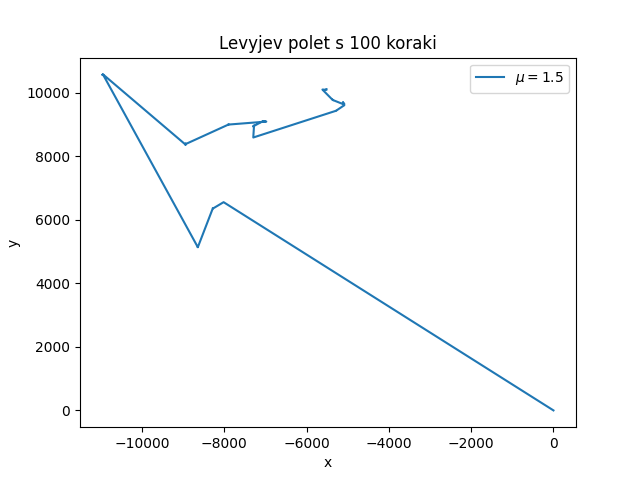
\includegraphics[width=0.95\textwidth]{sprehodi/let-100-1.5.png}
	\caption{2D polet s 100 koraki pri $\mu = 1.5$.}
	\label{fig-let-100-1.5}
\end{subfigure}
\begin{subfigure}{0.49\textwidth}
	\centering
	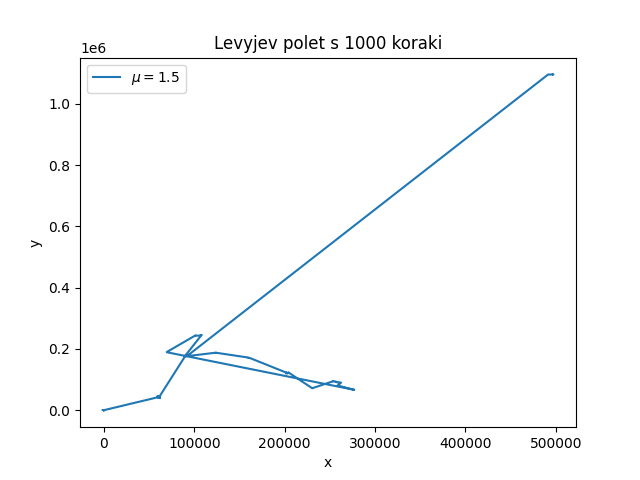
\includegraphics[width=0.95\textwidth]{sprehodi/let-1000-1.5.png}
	\caption{2D polet s 1000 koraki pri $\mu = 1.5$.}
	\label{fig-let-1000-1.5}
\end{subfigure}
\begin{subfigure}{0.49\textwidth}
	\centering
	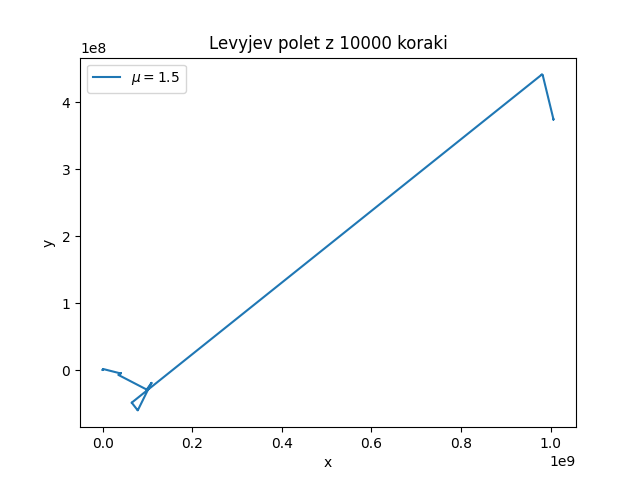
\includegraphics[width=0.95\textwidth]{sprehodi/let-10000-1.5.png}
	\caption{2D polet z 10000 koraki pri $\mu = 1.5$.}
	\label{fig-let-10000-1.5}
\end{subfigure}

\begin{subfigure}{0.49\textwidth}
	\centering
	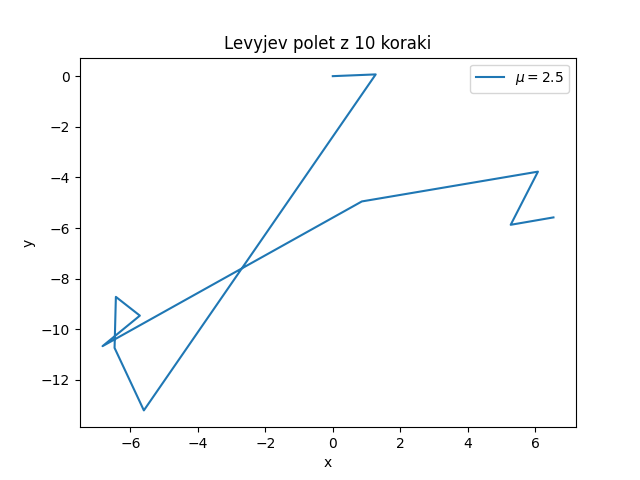
\includegraphics[width=0.95\textwidth]{sprehodi/let-10-2.5.png}
	\caption{2D polet z 10 koraki pri $\mu = 2.5$.}
	\label{fig-let-10-2.5}
\end{subfigure}
\begin{subfigure}{0.49\textwidth}
	\centering
	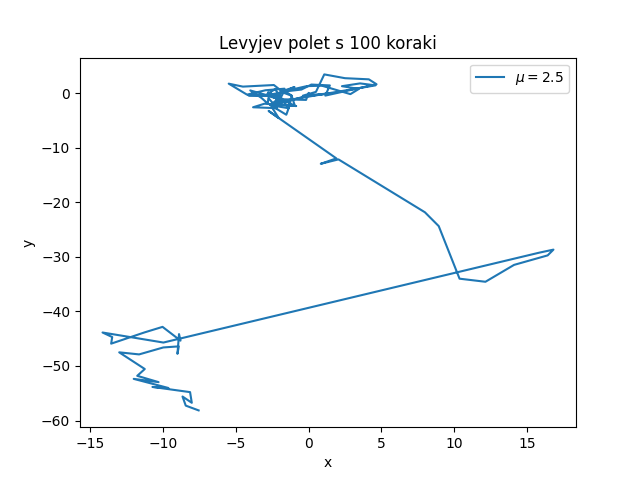
\includegraphics[width=0.95\textwidth]{sprehodi/let-100-2.5.png}
	\caption{2D polet s 100 koraki pri $\mu = 2.5$.}
	\label{fig-let-100-2.5}
\end{subfigure}
\end{figure}
\begin{figure}[H]
\ContinuedFloat
\begin{subfigure}{0.49\textwidth}
	\centering
	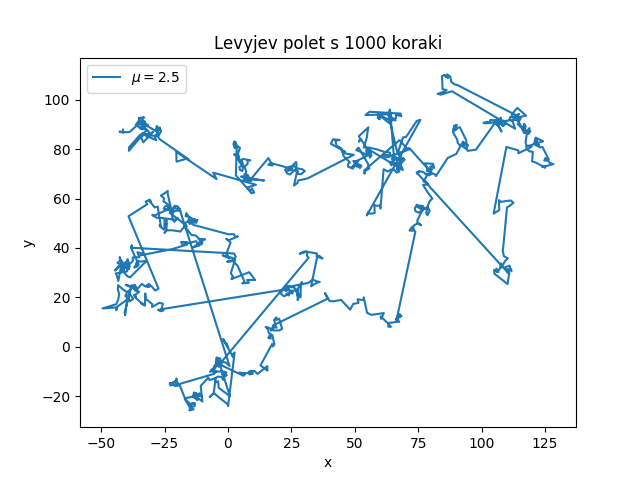
\includegraphics[width=0.95\textwidth]{sprehodi/let-1000-2.5.png}
	\caption{2D polet s 1000 koraki pri $\mu = 2.5$.}
	\label{fig-let-1000-2.5}
\end{subfigure}
\begin{subfigure}{0.49\textwidth}
	\centering
	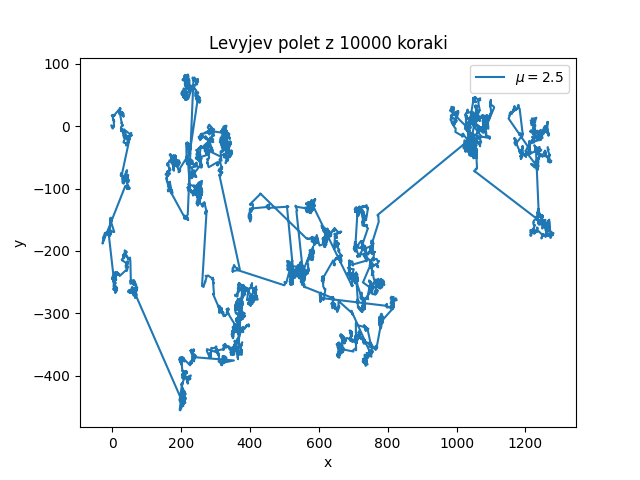
\includegraphics[width=0.95\textwidth]{sprehodi/let-10000-2.5.png}
	\caption{2D polet z 10000 koraki pri $\mu = 2.5$.}
	\label{fig-let-10000-2.5}
\end{subfigure}

\begin{subfigure}{0.49\textwidth}
	\centering
	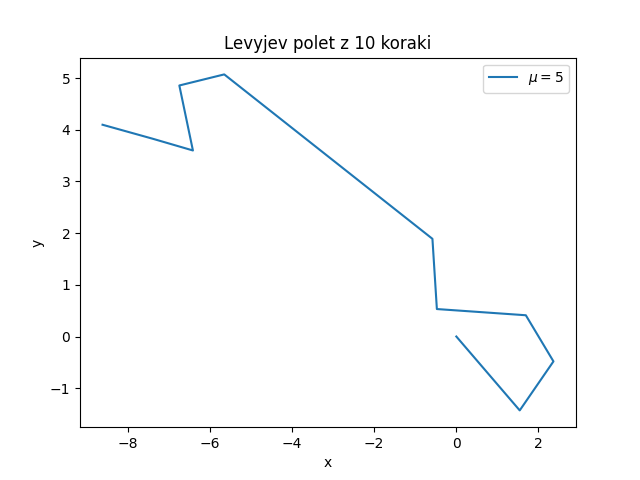
\includegraphics[width=0.95\textwidth]{sprehodi/let-10-5.png}
	\caption{2D polet z 10 koraki pri $\mu = 5$.}
	\label{fig-let-10-5}
\end{subfigure}
\begin{subfigure}{0.49\textwidth}
	\centering
	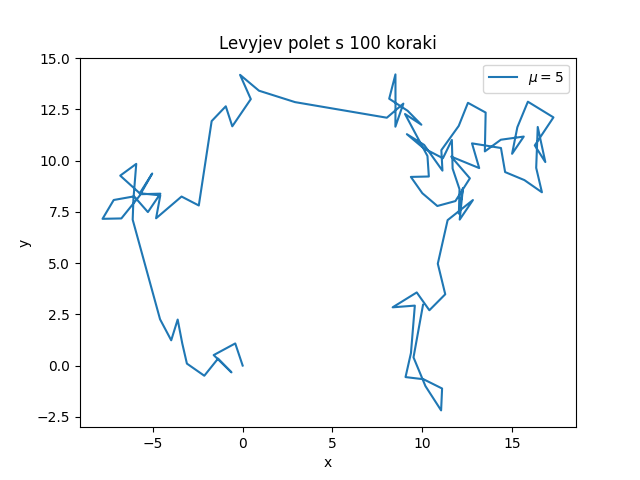
\includegraphics[width=0.95\textwidth]{sprehodi/let-100-5.png}
	\caption{2D polet s 100 koraki pri $\mu = 5$.}
	\label{fig-let-100-5}
\end{subfigure}
\begin{subfigure}{0.49\textwidth}
	\centering
	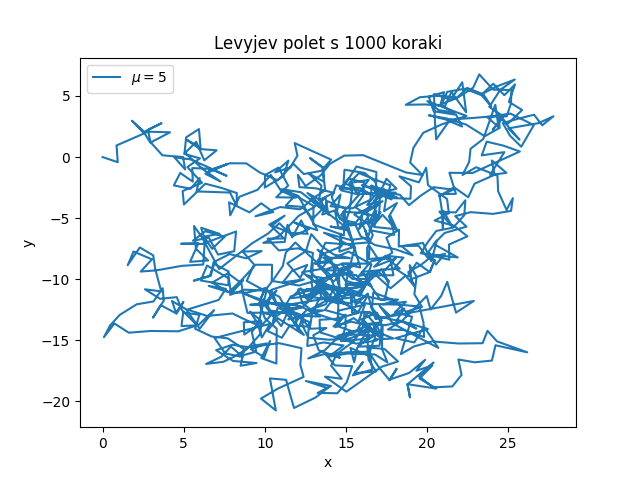
\includegraphics[width=0.95\textwidth]{sprehodi/let-1000-5.png}
	\caption{2D polet s 1000 koraki pri $\mu = 5$.}
	\label{fig-let-1000-5}
\end{subfigure}
\begin{subfigure}{0.49\textwidth}
	\centering
	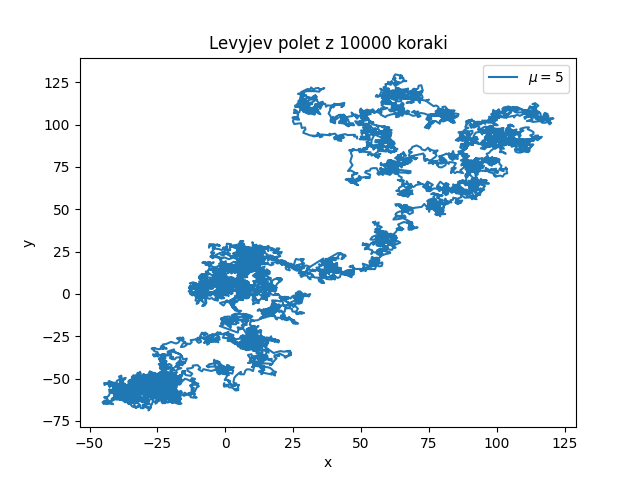
\includegraphics[width=0.95\textwidth]{sprehodi/let-10000-5.png}
	\caption{2D polet z 10000 koraki pri $\mu = 5$.}
	\label{fig-let-10000-5}
\end{subfigure}

\caption{Trajektorije 2D Levyjevih poletov za različno število korakov in različne vrednosti $\mu$.}
\label{fig-leti}
\end{figure}

Opazimo, da vse trajektorije načeloma izgledajo podobno. Pri manjših eksponentih $\mu$ je večja verjetnost za ekstremno dolge korake, ki vizualno razbijejo trajektorije. Pri vrednosti $\mu = 1.5$, imajo dolgi koraki prevelik vpliv, da bi bile slike uporabne. Nasprotno pa je na malo manj ekstremni sliki \ref{fig-let-10000-2.5} zelo dobro vidna fragmentacija trajektorije zaradi daljših korakov. Pri večjih vrednostih $\mu=5$ pa je slika bolj povezana.



\section{Vzporedni eksperimenti}
V tem delu naloge bom vzporedno izvajal več sprehodov in jih primerjal med sabo. Pri poletih je to enostavno, saj med vsakim korakom poteče enako časa. Paziti moramo le na to, da pri sprehodih, kjer je trajanje med vsakim korakom različno, gledamo kaj se dogaja na konstantnih časovnih intervalih.	\par\vspace{5mm}

Gledal bom odstopanja med vzporednimi poskusi. Drugi moment Pareto porazdelitve je neskončen, zato vsota za izračun $\sigma$ slabo konvergira. Namesto tega bom uporabil MAD, ki je bol robusten operator in manj občutljiv na oddaljene vrednosti. ker je kot za vse korake enakomerno naključno prazdeljen, naj bi bili sprehodi simetrični v $x$ in $y$ dimenziji po dolgem času. Zato ju bom obravnaval kar skupaj.\par\vspace{5mm}

S pomočjo drugega momenta gibanj bom določil eksponent $\gamma$. Opravil bom 1000 vzporednih poskusov s 1000 koraki za tri različne eksponente $\mu$. Narisal bom graf meritev, kjer bom gledal odvisnost log(MAD) od logaritma časa (korakov). V tej skali lahko za vsak set meritev določim premico s pomočjo linearne regresije (\texttt{scipy.curvefit}).

\begin{figure}[H]
\centering
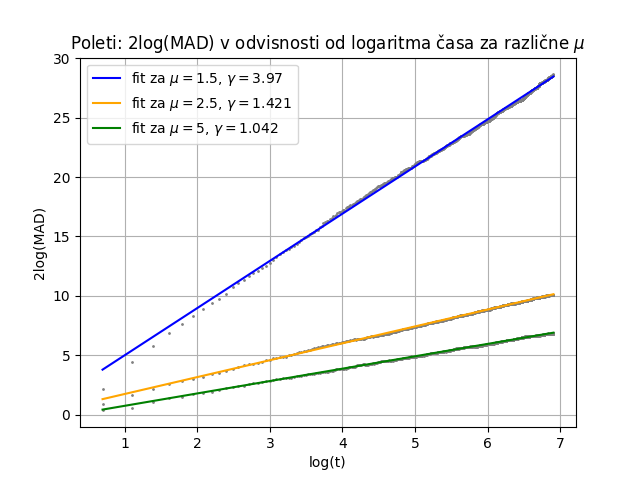
\includegraphics[width=0.7\textwidth]{grafi/polet-1000-1000.png}
\caption{Graf meritev log(MAD) za tisoč vzporednih poletov tisoč koraki za $\mu = 1.5$, 2.5, 5. Prikazane so tudi fitane premice s koeficienti $\gamma$.}
\label{fig-poleti-gamma}
\end{figure} 

Na slikah \ref{fig-poleti-gamma}  in \ref{fig-sprehodi-gamma} so narisane linearne regresije za polete in sprehode z istimi prametri. Opazno je, da nakloni premic pri poletih z naraščanjem koeficienta $\mu$ hitreje rastejo. To je posledica tega, da se delci pri sprehodu gibljejo s konstantno hitrostjo, pri poletu pa lahko v zelo kratkem času skočijo zelo daleč.

\begin{figure}[H]
\centering
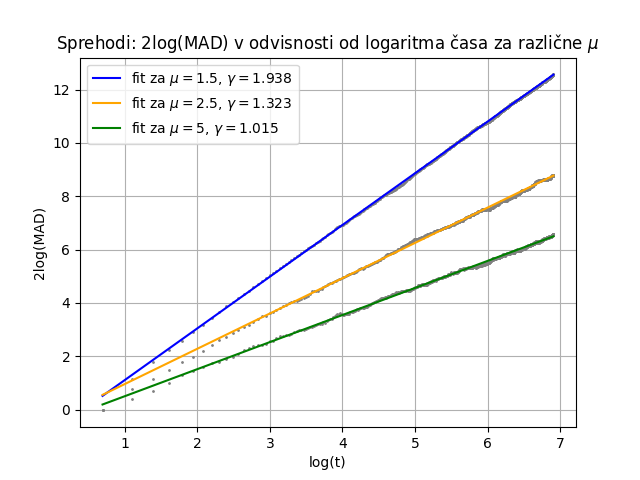
\includegraphics[width=0.7\textwidth]{grafi/sprehod-1000-1000.png}
\caption{Graf meritev log(MAD) za tisoč vzporednih sprehodov tisoč koraki za $\mu = 1.5$, 2.5, 5. Prikazane so tudi fitane premice s koeficienti $\gamma$.}
\label{fig-sprehodi-gamma}
\end{figure} \par\vspace{5mm}


Razliko med obnašanjem $\gamma$ za sprehode in polete bo najlažje videti, če narišem graf $\gamma(\mu)$ za obe vrsti gibanja (slika\ref{fig-gamma}). Svoje rezultate bom primerjal še s teoretično napovedjo.

\begin{figure}[H]
\centering
\begin{subfigure}{0.49\textwidth}
	\centering
	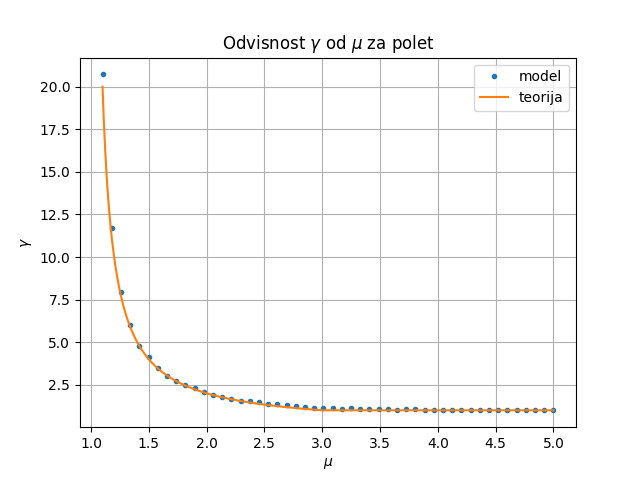
\includegraphics[width=0.95\textwidth]{grafi/gamma-poleti.png}
	\caption{Polet. Do $\mu = 3$ super-difuzivni režim ($\gamma = \frac{2}{\mu-1}$), $\mu>3$ normalna difuzija.}
	\label{fig-gmul}
\end{subfigure}
\begin{subfigure}{0.49\textwidth}
	\centering
	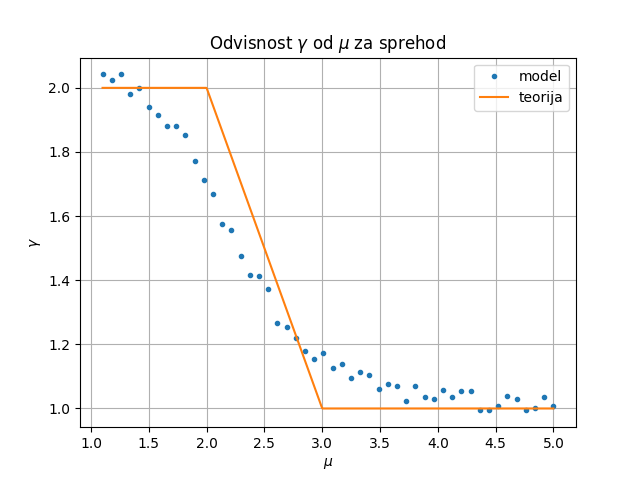
\includegraphics[width=0.95\textwidth]{grafi/gamma-sprehodi.png}
	\caption{Sprehod. Do $\mu = 2$ balistični režim, $2<\mu<3$ super-difuzivni režim ($\gamma = 4-\mu$), $\mu>3$ normalna difuzija.}
	\label{fig-gmus}
\end{subfigure}
\caption{Grafa odvisnosti $\gamma(\mu)$ za polete in sprehode. Spet vsakič za 1000 poskusov s 1000 koraki za 50 različnih $\mu$.}
\label{fig-gamma}
\end{figure} \par\vspace{5mm}

Pri poletih (slika \ref{fig-gmul}) se model super prilagaja teoriji. Vidimo tudi, da $\gamma$ pri majhnih vrednostih divergira, kar je skladno z opazkami iz prejšnjega odstavka. Model sprehoda se teoretični napovedi prilagaja dokaj slabše. Graf ni dovolj stopničast in vrednosti narastejo tudi čez 2, kamor bi morale konvergirati.


\section{Zaključek}
Model Levyjevih sprehodov in poletov mi je dal smiselne rezultate. Grafi so prav tako logični in se ujemajo med seboj. Edini primer, ko model ni bil res natančen je pri $\gamma(\mu)$ za sprehode. Domnevam, da je do tega prišlo zaradi stopničastosti teoretične napovedi. Verjetno bi se ji lahko bolj približal, če bi opravil še več meritev. 








\begin{thebibliography}{99}
\setlength{\itemsep}{.2\itemsep}\setlength{\parsep}{.5\parsep}
\bibitem{weeks} E.~R.~Weeks, J.~S.~Urbach, H.~L.~Swinney, Physica D {\bf 97} (1996) 291.
\end{thebibliography}

\end{document}
